\section{Ice Model Formulation}
\label{Iphys}

Hibler \cite{Hibler79} has described a model for the simulation of sea
ice circulation and thickness.  The model has been tested over a
seasonal cycle and the results are also shown in that article.  This
report was derived from the documentation for the sea ice model written
by Hibler \cite{HiblerDoc} since the dynamical equations are much the
same.  The model itself has been rewritten by Paul Budgell and is now
implemented on an orthogonal, curvilinear Arakawa C-grid, has a new
elliptic solver, and the nonlinear advection of momentum has been
omitted.  The thermodynamics are derived from Mellor and Kantha
\cite{Mellor89} (MK89 below). Sirpa H\"akkinen allowed us to use her
implementation of MK89; we obtained it from the Norwegians, who call it
``hakkis''.

\subsection{Model structure}
The overall structure consists of two principal components---the
momentum equations and the ice continuity equations.  The momentum
balance includes air and water stress, Coriolis force, internal ice
stress, inertial forces and ocean tilt as shown in equations
(\ref{ist1}) and (\ref{ist2}):
\begin{align}
  M {\partial u \over \partial t}
 % + M \vec{v} \cdot \nabla u
 & = Mfv - Mg {\partial \zeta_w \over \partial x} +
 \tau_a^x + \tau_w^x + {\cal F}_x
\label{ist1} \\
  M {\partial v \over \partial t}
 % + M \vec{v} \cdot \nabla v
 & = - Mfu - Mg {\partial \zeta_w \over \partial y} +
 \tau_a^y + \tau_w^y + {\cal F}_y.
\label{ist2}
\end{align}
In this model, we neglect the nonlinear advection terms as well as
the curvilinear terms in the internal ice stress.
Nonlinear formulas are used for both the ocean-ice and air-ice surface
stress:
\begin{align}
  \vec{\tau}_a & = \rho_a C_a | \vec{V}_{10} | \vec{V}_{10} \\
  C_a & = {1 \over 2} C_d \left[ 1 - \cos( 2 \pi \min(h_i+.1, .5)
  \right] \\
  \vec{\tau}_w & = \rho_w C_w | \vec{v}_w - \vec{v} |
  ( \vec{v}_w - \vec{v}) .
\end{align}
The force due to
the internal ice stress is given by the divergence of the stress
tensor $\sigma$. The rheology is given by the stress-strain relation
of the medium. We would like to emulate the viscous-plastic rheology
of Hibler (1979) \cite{Hibler79}:
\begin{equation}
  \sigma_{ij} = 2 \eta \dot \epsilon_{ij} + (\zeta - \eta) \dot
  \epsilon_{kk} \delta_{ij} - {P \over 2} \delta_{ij}
\end{equation}
\begin{equation}
  \dot \epsilon_{ij} \equiv {1 \over 2} \left( {\partial u_i \over
  \partial x_j} + {\partial u_j \over \partial x_i} \right)
\end{equation}
\begin{equation}
  P = P^* A h_i e^{-C(1-A)}
\end{equation}
where the nonlinear viscosities are given by
\begin{equation}
\zeta = { P \over 2 \left[ (\epsilon^2_{11} +
   \epsilon^2_{22} ) ( 1 + 1/e^2 ) + 4 e^{-2} \epsilon^2_{12}
      + 2 \epsilon_{11} \epsilon_{22} ( 1 - 1/e^2 ) \right] ^{1/2} }
\end{equation}
\begin{equation}
      \eta = { \zeta \over e^2 }.
\end{equation}
We would also like to have an explicit model that can be solved
efficiently on parallel computers. The EVP rheology has a tunable
coefficient $E$ (the Young's modulus) which can be chosen to make
the elastic term small compared to the other terms. We rearrange the VP
rheology:
\begin{equation}
  {1 \over 2 \eta} \sigma_{ij} + {\eta - \zeta \over 4 \eta \zeta}
  \sigma_{kk} \delta_{ij} + {P \over 4 \zeta} \delta_{ij} = \dot
  \epsilon_{ij}
\end{equation}
then add the elastic term:
\begin{equation}
  {1 \over E} {\partial \sigma_{ij} \over \partial t} + {1 \over 2
  \eta} \sigma_{ij} + {\eta - \zeta \over 4 \eta \zeta} \sigma_{kk}
  \delta_{ij} + {P \over 4 \zeta} \delta_{ij} = \dot \epsilon_{ij}
\end{equation}

Much like the ocean model, the ice model has a split timestep. The
internal ice stress term is updated on a shorter timestep so as to
allow the elastic wave velocity to be resolved.

Once the new ice velocities are computed, the ice tracers can be
advected using the MPDATA scheme \cite{Smolarkiewicz}. The tracers in
this case are the ice thickness, ice concentration, snow thickness,
internal ice temperature, and surface melt ponds. The continuity
equations describing the evolution of these parameters (equations
(\ref{ist3a})--(\ref{ist3b})) also include thermodynamic terms ($S_h$,
$S_s$ and $S_A$), which will be described in \S\ref{Growth}:
\begin{align}
  {\partial A h_i \over \partial t} & =
  - {\partial (u A h_i) \over \partial x} -
  {\partial (v A h_i) \over \partial y}
  + S_h + {\cal D}_h
\label{ist3a} \\
  {\partial A h_s \over \partial t} & =
  - {\partial (u A h_s) \over \partial x} -
  {\partial (v A h_s) \over \partial y}
  + S_s + {\cal D}_s
\label{ist3c} \\
  {\partial A \over \partial t} & =
  - {\partial (uA) \over \partial x} - {\partial (vA) \over \partial y}
  + S_A + {\cal D}_A \qquad \qquad 0 \leq A \leq 1 .
\label{ist3b}
\end{align}
The first two equations represent the conservation of ice and snow.
Equation \ref{ist3b} is discussed in some detail in MK89, but
represents the advection of ice blocks in which no ridging occurs as
long as there is any open water. An optional ridging term can be added
(Gray and Killworth \cite{Gray96}):
\begin{equation}
  {\partial A \over \partial t} =
  - {\partial (uA) \over \partial x} - {\partial (vA) \over \partial y}
  - A \alpha(A) \, \nabla \cdot \vec{v} \, H(-\nabla \cdot \vec{v})
  + S_A + {\cal D}_A \qquad \qquad 0 \leq A \leq 1 .
\end{equation}
where $\alpha(A)$ is an arbitrary function such that $\alpha(0) = 0$,
$\alpha(1) = 1$, and $0 \leq \alpha(A) \leq 1$. The ridging term leads
to an increase in $h_i$ under convergent flow as would be produced by
ridging. The function $\alpha(A)$ should be chosen so that it is near
zero until the ice concentration is large enough that ridging is
expected to occur, then should increase smoothly to one.

The symbols used in these equations along with the values for the
constants are listed in Table \ref{icemomvars}.

\begin{table}[pt]
\hspace{9.5 mm}
\vbox{
\begin{tabular}{|c|c|l|} \hline
  Variable & Value & Description \\ \hline
  $A(x,y,t)$ && ice concentration \\
  $\alpha(A)$ && ridging function \\
  $C_a$ && nonlinear air drag coefficient \\
  $C_d$ & $2.2 \times 10^{-3}$ & air drag coefficient \\
  $C_w$ & $10 \times 10^{-3}$ & water drag coefficient \\
  (${\cal D}_h, {\cal D}_s, {\cal D}_A$) && diffusion terms \\
  $\delta_{ij}$ && Kronecker delta function \\
  $E$ && Young's modulus \\
  $e$ & 2 & eccentricity of the elliptical yield curve \\
  $\epsilon_{ij}(x,y,t)$ && strain rate tensor \\
  $\eta(x,y,t)$ && nonlinear shear viscosity \\
  $f(x,y)$ && Coriolis parameter \\
  (${\cal F}_x, {\cal F}_y$) && internal ice stress \\
  $g$  & $9.8\, m\, s^{-2}$ & acceleration of gravity \\
  $H$ &&  Heaviside function \\
  $h_i(x,y,t)$ && ice thickness of ice-covered fraction \\
  $h_o$ & 1 m & ice cutoff thickness \\
  $h_s(x,y,t)$ && snow thickness on ice-covered fraction \\
  $M(x,y,t)$ && ice mass (density times thickness) \\
  $P(x,y,t)$ && ice pressure or strength \\
  ($P^*, C$) & ($2.75 \times 10^4, 20$) & ice strength parameters \\
  ($S_h, S_s, S_A$) && thermodynamic terms \\
  $\sigma_{ij}(x,y,t)$ && stress tensor \\
  $\vec{\tau}_a$ && air stress \\
  $\vec{\tau}_w$ && water stress \\
  ($u,v$) && the ($x,y$) components of ice velocity $\vec{v}$ \\
  ($\vec{V}_{10}, \vec{v}_w$) &&
	      10 meter air and surface water velocities \\
  ($\rho_a, \rho_w$)  & ($1.3\, kg\, m^{-3}, 1025\, kg\, m^{-3}$) & air
  and water densities \\
  $\zeta(x,y,t)$ && nonlinear bulk viscosity \\
  $\zeta_w(x,y,t)$ && height of the ocean surface \\
  \hline
\end{tabular}
}
\caption{Variables used in the ice momentum equations}
\label{icemomvars}
\end{table}

%The viscous-plastic terms (\ref{fx1}) and (\ref{fy1})
%are found by taking the divergence of the stress tensor:
%\begin{equation}
%  ({\cal F}_x, {\cal F}_y) = \nabla \cdot \mbox{\boldmath $\sigma$}
%\end{equation}
%with the result that
%\begin{equation}
%   {\cal F}_x = {\partial \over \partial x} \left[ (\eta + \zeta)
%   {\partial u \over \partial x} + (\zeta - \eta)
%   {\partial v \over \partial y} - P/2 \right] +
%   {\partial \over \partial y} \left[ \eta \left( 
%   {\partial u \over \partial y} + {\partial v \over \partial x}
%   \right) \right]
%\label{fx1}
%\end{equation}
%\begin{equation}
%   {\cal F}_y = {\partial \over \partial y} \left[ (\eta + \zeta)
%   {\partial v \over \partial y} + (\zeta - \eta)
%   {\partial u \over \partial x} - P/2 \right] +
%   {\partial \over \partial x} \left[ \eta \left( 
%   {\partial u \over \partial y} + {\partial v \over \partial x}
%   \right) \right]
%\label{fy1}
%\end{equation}

%The ``pressure gradient'' term is also modeled as a term in the
%internal ice stress.  This term represents the resistance which ice
%has to being compressed (ice strength) and is a function of ice
%thickness and concentration:
%\begin{equation}
%  P = P^* A h_i \exp[ -C (1-A)] H(-\nabla \cdot \vec{v})~.
%\label{press}
%\end{equation}
%The Heaviside function guarantees that the ice has no strength when the
%flow is divergent (Gray and Killworth \cite{Gray95}).

\subsection{Horizontal curvilinear coordinates}

Applying the curvilinear transformation used in \S\ref{Ocurve} and
described in Appendix \ref{Curve}, we use a transformation to an
orthogonal curvilinear coordinate system.  Denoting the velocity
components in the new coordinate system by
\begin{equation}
   \vec{v} \cdot \hat{\xi} = u
\end{equation}
and
\begin{equation}
   \vec{v} \cdot \hat{\eta} = v
\end{equation}
the equations of motion (\ref{ist1}), (\ref{ist2}),
(\ref{ist3a})--(\ref{ist3b}) can be re-written
(see, e.g., Arakawa and Lamb \cite{AL}):
{\samepage
%\[
 %  {\partial u \over \partial t}
 %  + m u {\partial u \over \partial \xi}
 %  + n v {\partial u \over \partial \eta}
 %  = \left\{f + mn \left[ v \frac{\partial}{\partial \xi}
 %  \!\! \left( \frac{1}{n} \right) - u \frac{\partial}{\partial \eta}
 %  \!\! \left( \frac{1}{m} \right) \right] \right\} v
%\]
\begin{equation}
   {\partial u \over \partial t} = fv
   - gm {\partial \zeta_w \over \partial \xi} +
   {1 \over M} \left( \tau_a^{\xi} + \tau_w^{\xi} + {\cal F}_{\xi}
   \right)
\label{ist13}
\end{equation}
}
\vspace{.2cm}
{\samepage
%\[
%   {\partial v \over \partial t} +
%   m u {\partial v \over \partial \xi} +
%   n v {\partial v \over \partial \eta} =
%   - \left\{f + mn \left[ v \frac{\partial}{\partial \xi}
%   \!\! \left( \frac{1}{n} \right) - u \frac{\partial}{\partial \eta}
%   \!\! \left( \frac{1}{m} \right) \right] \right\} u
%\]
\begin{equation}
   {\partial v \over \partial t} = - fu
   - gn {\partial \zeta_w \over \partial \eta} +
   {1 \over M} \left( \tau_a^{\eta} + \tau_w^{\eta} + {\cal F}_{\eta}
   \right)
\label{ist14}
\end{equation}
}
\begin{equation}
   {\partial A h_i \over \partial t} =
   - mn \left[ {\partial \over \partial \xi} \!\!
   \left( {A h_i u \over n}
   \right ) + {\partial \over \partial \eta} \!\!
   \left( {A h_i v \over m}
   \right) \right] + S_h
\label{ist15}
\end{equation}
\begin{equation}
   {\partial A h_s \over \partial t} =
   - mn \left[ {\partial \over \partial \xi} \!\!
   \left( {A h_s u \over n}
   \right ) + {\partial \over \partial \eta} \!\!
   \left( {A h_s v \over m}
   \right) \right] + S_s
\label{ist15a}
\end{equation}
\begin{equation}
   {\partial A \over \partial t} =
   - mn \left[ {\partial \over \partial \xi} \!\! \left( {Au \over n}
   \right ) + {\partial \over \partial \eta} \!\! \left( {Av \over m}
   \right) \right] + S_A
\label{ist16}
\end{equation}
\vspace{.2cm}
$S_h$, $S_s$ and $S_A$ remain unchanged.

The viscous-plastic terms can be derived from equation
(\ref{stress1}).  In curvilinear coordinates the strain rate tensor
can be written as:
\begin{equation}
   \epsilon_{11} = m {\partial u \over \partial \xi} +
    vmn {\partial \over \partial \eta} \!\! \left( {1 \over m} \right)
\end{equation}
\begin{equation}
   \epsilon_{12} = e_{21} = {1 \over 2} \left[
   {m \over n} {\partial \left( nv \right) \over \partial \xi}
   + {n \over m} {\partial \left( mu \right) \over \partial \eta}
   \right]
\end{equation}
\begin{equation}
   \epsilon_{22} = n {\partial v \over \partial \eta} +
    umn {\partial \over \partial \xi} \!\! \left( {1 \over n} \right)
\end{equation}
In curvilinear coordinates the divergence of a symmetric tensor {\bf T}
is:
\[
    \nabla \cdot \mbox{\bf T} =
    \hat{\xi} \left[ m
    {\partial \mbox{\bf T}_{11} \over \partial \xi}
    + n {\partial \mbox{\bf T}_{12} \over \partial \eta}
    + \mbox{\bf T}_{11} mn {\partial \over \partial \xi} \!\!
    \left( {1 \over n} \right) \right. \mbox{\hspace{2 cm}}
\]
\[
    \mbox{\hspace{2 cm}} \left. + 2 \mbox{\bf T}_{12} mn
    {\partial \over \partial \eta} \!\! \left( {1 \over m} \right)
    - \mbox{\bf T}_{22} mn
    {\partial \over \partial \xi} \!\! \left( {1 \over n} \right)
    \right]
\]
\[
    + \hat{\eta} \left[ m
    {\partial \mbox{\bf T}_{12} \over \partial \xi}
    + n {\partial \mbox{\bf T}_{22} \over \partial \eta}
    - \mbox{\bf T}_{11} mn {\partial \over \partial \eta} \!\!
    \left( {1 \over m} \right) \right. \mbox{\hspace{2 cm}}
\]
\begin{equation}
    \mbox{\hspace{2 cm}} \left. + 2 \mbox{\bf T}_{12} mn
    {\partial \over \partial \xi} \!\! \left( {1 \over n} \right)
    + \mbox{\bf T}_{22} mn
    {\partial \over \partial \eta} \!\! \left( {1 \over m} \right)
    \right]
\end{equation}
A more general expression for derivatives of tensors is given by
Aris \cite{Aris} in terms of Christoffel symbols.

The viscous-plastic terms become:
\[
   {\cal F}_{\xi} = m {\partial \over \partial \xi} \left[
   (\zeta - \eta ) mn {\partial \over \partial \xi} \!\! \left(
   {u \over n} \right) \right] +
   m {\partial \over \partial \xi} \left[
   (\zeta - \eta ) mn {\partial \over \partial \eta} \!\! \left(
   {v \over m} \right) \right] - {m \over 2}
   {\partial P \over \partial \xi}
\]
\[
   + 2 m {\partial \over \partial \xi} \left[ \eta m
   {\partial u \over \partial \xi} + \eta v mn 
   {\partial \over \partial \eta} \!\! \left( {1 \over m} \right)
   \right]
   + n {\partial \over \partial \eta} \left[ \eta {m \over n}
   {\partial (nv) \over \partial \xi} + \eta {n \over m}
   {\partial (mu) \over \partial \eta} \right]
\]
\[
   + 2 \eta m^2 n {\partial u \over \partial \xi}
   {\partial \over \partial \xi} \!\! \left( {1 \over n} \right)
   + 2 \eta v m^2 n^2
   {\partial \over \partial \eta} \!\! \left( {1 \over m} \right)
   {\partial \over \partial \xi} \!\! \left( {1 \over n} \right)
   + 2 \eta m^2 {\partial (nv) \over \partial \xi}
   {\partial \over \partial \eta} \!\! \left( {1 \over m} \right)
\]
\begin{equation}
   + 2 \eta n^2 {\partial (mu) \over \partial \eta}
   {\partial \over \partial \eta} \!\! \left( {1 \over m} \right)
   - 2 \eta m n^2 {\partial v \over \partial \eta}
   {\partial \over \partial \xi} \!\! \left( {1 \over n} \right)
   - 2 \eta u m^2 n^2 \left[
   {\partial \over \partial \xi} \!\! \left( {1 \over n} \right)
   \right]^2
\end{equation}
\vspace{2 mm}
\[
   {\cal F}_{\eta} = n {\partial \over \partial \eta} \left[
   (\zeta - \eta ) mn {\partial \over \partial \xi} \!\! \left(
   {u \over n} \right) \right] +
   n {\partial \over \partial \eta} \left[
   (\zeta - \eta ) mn {\partial \over \partial \eta} \!\! \left(
   {v \over m} \right) \right] - {n \over 2}
   {\partial P \over \partial \eta}
\]
\[
   + m {\partial \over \partial \xi} \left[ \eta {m \over n}
   {\partial (nv) \over \partial \xi} + \eta {n \over m}
   {\partial (mu) \over \partial \eta} \right]
   + 2n {\partial \over \partial \eta} \left[ \eta n
   {\partial v \over \partial \eta} + \eta u mn 
   {\partial \over \partial \xi} \!\! \left( {1 \over n} \right)
   \right]
\]
\[
   - 2 \eta m^2 n {\partial u \over \partial \xi}
   {\partial \over \partial \eta} \!\! \left( {1 \over m} \right)
   - 2 \eta v m^2 n^2 \left[
   {\partial \over \partial \eta} \!\! \left( {1 \over m} \right)
   \right]^2
   + 2 \eta m^2 {\partial (nv) \over \partial \xi}
   {\partial \over \partial \xi} \!\! \left( {1 \over n} \right)
\]
\begin{equation}
   + 2 \eta n^2 {\partial (mu) \over \partial \eta}
   {\partial \over \partial \xi} \!\! \left( {1 \over n} \right)
   + 2 \eta m n^2 {\partial v \over \partial \eta}
   {\partial \over \partial \eta} \!\! \left( {1 \over m} \right)
   + 2 \eta u m^2 n^2
   {\partial \over \partial \eta} \!\! \left( {1 \over m} \right)
   {\partial \over \partial \xi} \!\! \left( {1 \over n} \right)
\end{equation}

\subsection{Numerical Scheme}

A key feature of the numerical scheme is a staggered grid, known as
the ``Arakawa C grid'', where the velocity is defined on the sides of a
grid box and variables such as thickness and viscosity are defined
at the center of the grid box, as shown in Fig.\ \ref{fcgr}.

Because of the strong ice interaction (which in this model is
dissipative in nature) the momentum equations are essentially
parabolic in form and hence have few numerical instability problems
over long-term integrations.  (While there are few numerical
problems, it should be emphasized that the dissipative ice
interaction terms are highly nonlinear and can lead to unstable flow
fields in the absence of water drag.  Such a feature is a physical
characteristic of plastic flow and not a numerical artifact).
However, in principle it is possible for the ice interaction to be
very small even though there may be a finite ice mass.  Under this
situation, the momentum advection terms could cause nonlinear
instabilities.  To ensure against such situations, Hibler put a lower
limit on the bulk viscosity parameter
(and hence indirectly shear viscosity as well). It is never
allowed to drop below $1.0 \times 10^7$ $kg/s$, a value which
negligibly modifies the ice drift.
% We have not found this to be
% necessary and therefore do not limit the viscosities.

Nonlinear instabilities over long-term integrations can also arise from
the nonlinear advection terms in the thickness continuity equations.
To avoid this problem, the advection terms in equations
(\ref{ist3a})--(\ref{ist3b}) can be computed with a choice of either
Smolarkiewicz's MPDATA (\cite{Smolark90}) or third-order upwind
(Leonard \cite{Leonard79}). See \S\ref{Advect} for a description of
these schemes. It may be possible to omit the diffusivity from these
equations if the forcing fields are sufficiently smooth.

\subsection{Horizontal boundary conditions}

As mentioned above, initial conditions at all points and ice
velocities at the boundaries are thereafter required to initiate the
integration of the system of equations forward in time.  The most
natural boundary condition is to take the ice velocity to be zero on
the boundaries.  This can be done either at a land boundary or at an
ocean location where there is no ice.  Note that the boundary
condition does not affect the ice motion in such circumstances since
in the absence of ice the strength is zero.  More generally, as long
as the ocean boundaries are removed from the ice edge, the coupled
nature of the model will cause a natural ice edge boundary condition
to be created.  However, it is also possible to form an ``open''
boundary condition by setting the strength equal to zero near a
boundary.  These gridboxes are called ``outflow cells'' in Hibler
\cite{Hibler79}.  In the Arctic simulations, these outflow cells
are used at the open edge near Greenland.

The boundary conditions on the momentum equations are to set $u$ and $v$
to zero at all boundaries, including islands.  This is accomplished
by the elliptic solver during the implicit timestep.

The ice and snow thickness and ice concentration equations have no-flux
boundary conditions imposed along the mask boundaries.  The outflow
cells contain a radiation condition if the velocity is outward and no
change if the velocity is inward.

The primary characteristic of the outflow cells is that the ice
strength goes to zero there.  The values of $P$, $\zeta$, and $\eta$
are all set to zero in outflow cells.

\subsection{Thermodynamics}
\label{Growth}

The thermodynamics used is based on the algorithm described in
Mellor and Kantha \cite{Mellor89}, who have a useful description of the
various melting and freezing processes, plus the coupling to a full
three-dimensional ocean. Their form of equations
(\ref{ist3a}) and (\ref{ist3b}) is:
\begin{align}
  {\partial A h_i \over \partial t} +
  {\partial (u A h_i) \over \partial x} +
  {\partial (v A h_i) \over \partial y}
  & = {\rho_o \over \rho_i} \left[ A (W_{io} - W_{ai}) + (1-A) W_{ao}
  + W_{fr} \right]
\label{ist4a} \\
  {\partial A \over \partial t} +
  {\partial (uA) \over \partial x} + {\partial (vA) \over \partial y}
  & = {\rho_o A \over \rho_i h_i} \left[ \Phi (1-A) W_{ao} + (1-A)
  W_{fr} \right] \qquad \qquad 0 \leq A \leq 1 .
\label{ist4b}
\end{align}
Here, the $W$ variables are the freeze or
melt rates as shown in Fig.\ \ref{fm+k} and Table \ref{thermvar}.  The
frazil ice growth $W_{fr}$ will be discussed further in
\S\ref{frazil}---note that it contributes to changes in $A$ as well as
to changes in $h_i$.  The other term that contributes to $A$ is
$W_{ao}$.  This term includes a factor $\Phi$ which Mellor and Kantha
set to different values depending on whether ice is melting or
freezing:
\begin{align}
    \Phi & = 4.0 \qquad\qquad W_{ao} \geq 0 \\
    \Phi & = 0.5 \qquad\qquad W_{ao} < 0 \\
\end{align}

\begin{figure}[ht]
\setlength{\unitlength}{0.00083300in}%
%
%\begin{picture}(6527,2507)(270,-5042)
\begin{picture}(6527,2507)(885,-5042)
%\thicklines
\put(1501,-2911){\line( 1, 0){3975}}
\put(1501,-4111){\line( 1, 0){3975}}
\put(1501,-2911){\line( 0,-1){1200}}
\put(6976,-4111){\line( 1, 0){1050}}
\put(6976,-2911){\line( 1, 0){1050}}
\put(6976,-2911){\line( 0,-1){1200}}
\put(5476,-2911){\line( 0,-1){1200}}
\put(2401,-4861){\vector( 0, 1){750}}
\put(3376,-4861){\vector( 0, 1){750}}
\put(6226,-3586){\vector( 0, 1){675}}
\put(4426,-4036){\vector( 0,-1){525}}
\put(2596,-3376){\vector( 1, 1){450}}
%\put(1501,-5056){\framebox(6525,2505){}}
\put(6121,-3886){\makebox(0,0)[lb]{$W_{ao}$}}
\put(4336,-4756){\makebox(0,0)[lb]{$W_{ro}$}}
\put(2416,-3586){\makebox(0,0)[lb]{$W_{ai}$}}
\put(3241,-5056){\makebox(0,0)[lb]{$W_{io}$}}
\put(2296,-5056){\makebox(0,0)[lb]{$W_{fr}$}}
\end{picture}
%\begin{picture}(0,0)(5346,0)
\begin{picture}(0,0)(5961,0)
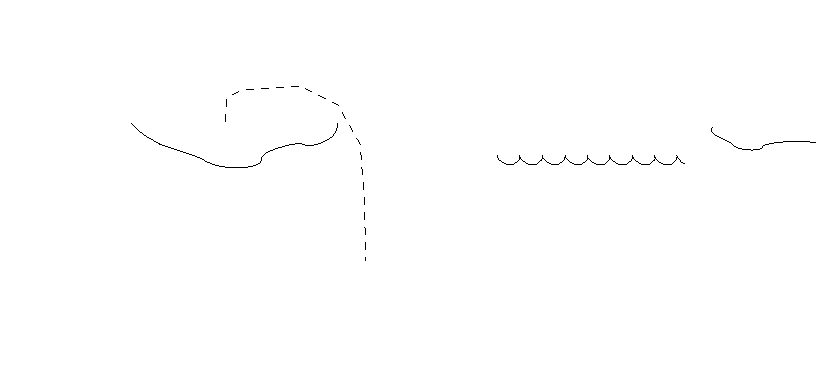
\includegraphics{pics/therm_mk}%
\end{picture}%
\caption{Diagram of the different locations where ice melting and
freezing can occur.}
\label{fm+k}
\end{figure}


\begin{table}
\hspace{9 mm}
\vbox{
\begin{tabular}{|c|c|l|} \hline
  Variable & Value & Description \\ \hline
  $\alpha_w$ & 0.10 & shortwave albedo of water \\
  $\alpha_i$ & 0.60 & shortwave albedo of wet ice \\
  $\alpha_i$ & 0.65 & shortwave albedo of dry ice \\
  $\alpha_s$ & 0.72 & shortwave albedo of wet snow \\
  $\alpha_s$ & 0.85 & shortwave albedo of dry snow \\
  $C_k$ && snow correction factor \\
  $C_{pi}$ & 2093 J kg$^{-1}$ K$^{-1}$ & specific heat of ice \\
  $C_{po}$ & 3990 J kg$^{-1}$ K$^{-1}$ & specific heat of water \\
  $\epsilon_w$ & 0.97 & longwave emissivity of water \\
  $\epsilon_i$ & 0.97 & longwave emissivity of ice \\
  $\epsilon_s$ & 0.99 & longwave emissivity of snow \\
  $E(T,r)$ && enthalpy of the ice/brine system \\
  $F_T\!\uparrow$ && heat flux from the ocean into the ice \\
  $H\!\downarrow$ && sensible heat \\
  $i_w$ && fraction of the solar heating transmitted \\
  && through a lead into the water below \\
  $k_i$ & 2.04 W m$^{-1}$ K${^-1}$ & thermal conductivity of ice \\
  $k_s$ & 0.31 W m$^{-1}$ K${^-1}$ & thermal conductivity of snow \\
  $L_i$ & 302 MJ m$^{-3}$ & latent heat of fusion of ice \\
  $L_s$ & 110 MJ m$^{-3}$ & latent heat of fusion of snow \\
  $LE\!\downarrow$ && latent heat \\
  $LW\!\!\downarrow$ && incoming longwave radiation \\
  $m$ & $-0.054^\circ$C/PSU & coefficient in linear $T_f(S) = mS$ equation \\
  $\Phi$ && contribution to $A$ equation from freezing water \\
  $Q_{ai}$ && heat flux out of the snow/ice surface \\
  $Q_{ao}$ && heat flux out of the ocean surface \\
  $Q_{i2}$ && heat flux up out of the ice \\
  $Q_{io}$ && heat flux up into the ice \\
  $Q_{s}$  && heat flux up through the snow \\
  $r$   && brine fraction in ice \\
  $\rho_i$ & 910 $m^3/kg$ & density of ice \\
  $S_i$ & 5 PSU & salinity of the ice \\
  $SW\!\!\downarrow$ && incoming shortwave radiation \\
  $\sigma$ & $5.67 \times 10^{-8}$ W m$^{-2}$ K$^{-4}$ &
  Stefan-Boltzmann constant \\
  $T_0$ && temperature of the bottom of the ice \\
  $T_1$ && temperature of the interior of the ice \\
  $T_2$ && temperature at the upper surface of the ice \\
  $T_3$ && temperature at the upper surface of the snow \\
  $T_f$ && freezing temperature \\
  $T_{{\rm melt}\_i}$ & $mS_i$ & melting temperature of ice \\
  $T_{{\rm melt}\_s}$ & 0$^\circ$ C & melting temperature of snow \\
  $W_{ai}$ && melt rate on the upper ice/snow surface \\
  $W_{ao}$ && freeze rate at the air/water interface \\
  $W_{fr}$ && rate of frazil ice growth \\
  $W_{io}$ && freeze rate at the ice/water interface \\
  $W_{ro}$ & $W_{ai}$ & rate of run-off of surface melt water \\
  \hline
\end{tabular}
}
\caption{Variables used in the ice thermodynamics}
\label{thermvar}
\end{table}

\begin{figure}
\centerline{
\begin{picture}(0,0)%
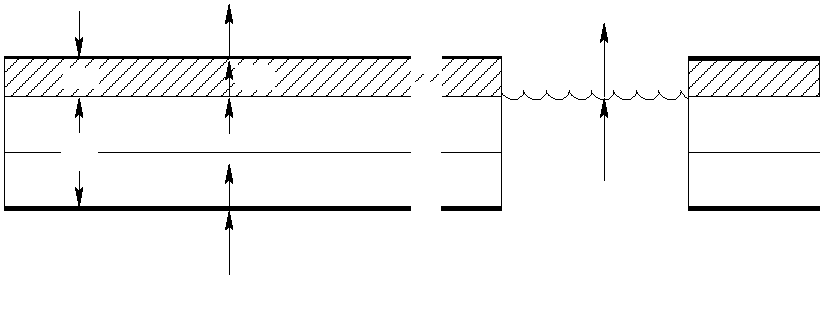
\includegraphics{pics/therm_mk2}%
\end{picture}%
\setlength{\unitlength}{3947sp}%
%
\begin{picture}(6591,2608)(1468,-5057)
\put(6376,-3511){\makebox(0,0)[lb]{{$F_T$}}}
\put(3376,-4561){\makebox(0,0)[lb]{{$F_T$}}}
\put(3376,-4036){\makebox(0,0)[lb]{{$Q_{io}$}}}
\put(3376,-3436){\makebox(0,0)[lb]{{$Q_{i2}$}}}
\put(6376,-3061){\makebox(0,0)[lb]{{$Q_{ao}$}}}
\put(3376,-3136){\makebox(0,0)[lb]{{$Q_s$}}}
\put(3376,-2761){\makebox(0,0)[lb]{{$Q_{ai}$}}}
\put(2026,-3736){\makebox(0,0)[lb]{{$h_i$}}}
\put(2026,-3136){\makebox(0,0)[lb]{{$h_s$}}}
\put(4801,-4186){\makebox(0,0)[lb]{{$T_0$}}}
\put(4801,-2986){\makebox(0,0)[lb]{{$T_3$}}}
\put(4801,-3286){\makebox(0,0)[lb]{{$T_2$}}}
\put(4801,-3736){\makebox(0,0)[lb]{{$T_1$}}}
\end{picture}
}
\caption{Diagram of internal ice temperatures and fluxes. The hashed
layer is the snow.}
\label{fflux}
\end{figure}

Figure \ref{fflux} shows the locations of the ice and snow temperatures
and the heat fluxes. The temperature profile is assumed to be linear
between adjacent temperature points. The interior of the ice contains
``brine pockets'', leading to a prognostic equation for the temperature
$T_1$.

The surface flux to the air is:
\begin{equation}
   Q_{ai} =  - H\!\downarrow - LE\!\downarrow -
       \epsilon_s LW\!\!\downarrow  -
      (1 - \alpha_s) SW\!\!\downarrow + \epsilon_s \sigma (T_3+273)^4
\end{equation}
The formulas for sensible heat, latent heat, and incoming longwave and
shortwave radiations are the same as in Parkinson and Washington
\cite{Parkinson} and
are shown in Appendix \ref{shortwave}. The sensible heat is a function
of $T_3$, as is the heat flux through the snow $Q_s$. Setting $Q_{ai} =
Q_s$, we can solve for $T_3$ by setting $T_3^{n+1} = T_3^n + \Delta
T_3$ and linearizing in $\Delta T_3$.  The temperature $T_3$ is found by
an iterative solution of the surface heat flux balance (using the
previous value of $T_1$ in equation \ref{qsnow}). As in Parkinson and
Washington, if $T_3$ is found to be above the melting temperature, it
is set to $T_{\rm melt}$ and the extra energy goes into melting the
snow or ice:
\begin{align}
   W_{ai} & = {Q_{ai} - Q_{i2} \over \rho_o L_3} \\
   L_3 & \equiv \left[ E(T_3,1) - E(T_1, R_1) \right]
\end{align}
Note that $L_3 = (1-r)L_i$ plus a small sensible heat correction.
We are not storing water on the surface in melt pools, so everything
melted at the surface is assumed to flow into the ocean ($W_{ro} =
W_{ai}$).

Inside the ice there are brine pockets in which there is salt water
at the {\it in situ} freezing temperature. It is assumed that the ice
has a uniform overall salinity of $S_i$ and that the freezing
temperature is a linear function of salinity. The brine fraction $r$ is
given by
$$
  r = {S_i m \over T_1}
$$
The enthalpy of the combined ice/brine system is given by
\begin{equation}
  E(T,r) = r(L_i + C_{po}T) + (1-r) C_{pi} T
\end{equation}
Substituting in for $r$ and differentiating gives:
\begin{equation}
  {\partial E \over \partial T} = - {S_i m L_i \over T_1^2} + C_{pi}
\end{equation}

Inside the snow, we have
\begin{equation}
   Q_s = {k_s \over h_s} (T_2 - T_3)
\end{equation}
The heat conduction in the upper part of the ice layer is
\begin{equation}
   Q_{I2} = { 2 k_i \over h_i} (T_1 - T_2)
   \label{qi2}
\end{equation}
These can be set equal to each other to solve for $T_2$
\begin{equation}
   T_2 = {T_3 + C_k T_1 \over 1 + C_k}
\end{equation}
where
$$
  C_k \equiv {2 k_i h_s \over h_i k_s}.
$$
Substituting into (\ref{qi2}), we get:
\begin{equation}
  Q_s = Q_{I2} = {2k_i \over h_i} {(T_1 - T_3) \over (1 + C_k)}
\label{qsnow}
\end{equation}
Note that in the absence of snow, $C_k$ becomes zero and we recover the
formula for the no-snow case in which $T_3 = T_2$.

At the bottom of the ice, we have
\begin{equation}
  Q_{I0} = {2 k_i \over h_i} (T_0 - T_1)
\end{equation}
The difference between $Q_{I0}$ and $Q_{I2}$ goes into the enthalpy of
the ice:
\begin{equation}
   \rho_i h_i \left[ {\partial E \over \partial t} + \vec{v} \cdot 
   \nabla E \right] = Q_{I0} - Q_{I2}
\end{equation}
We can use the chain rule to obtain an equation for timestepping $T_1$:
\begin{equation}
   \rho_i h_i {\partial E \over \partial T}
   \left[ {\partial T_1 \over \partial t} + \vec{v} \cdot 
   \nabla T_1 \right] = Q_{I0} - Q_{I2}
\end{equation}
where
\begin{align*}
  Q_{I0} - Q_{I2} & = {2 k_i \over h_i} \left[ (T_0 - T_1) - 
  {(T_1 - T_3) \over 1 + C_k} \right] \\
	          & = {2 k_i \over h_i} \left[ (T_0 +
  {T_3 - (2 + C_k) T_1 \over 1 + C_k} \right]
\end{align*}

\subsubsection{Ocean surface boundary conditions}
The ocean receives surface stresses from both the atmosphere and the
ice, according to the ice concentration:
\begin{align}
   K_m {\partial u_w \over \partial z} & = {A \over \rho_o} \tau_{io}^x
    + {1-A \over \rho_o} \tau_{ao}^x \\
   K_m {\partial v_w \over \partial z} & = {A \over \rho_o} \tau_{io}^y
    + {1-A \over \rho_o} \tau_{ao}^y
\end{align}
where the relevant variables are in table \ref{tobc}.

\begin{table}
\hspace{35 mm}
\vbox{
\begin{tabular}{|c|c|l|} \hline
Variable & Value & Definition \\ \hline
   $b$ & 3.0 & factor \\
   \.E && evaporation \\
   $k$ & 0.4 & von Karman's constant \\
   $\nu$ & $1.8 \times 10^{-6} m^2 s^{-1}$ &
      kinematic viscosity of seawater \\
   \.P && precipitation \\
   $Pr$ & 13.0 & molecular Prandtl number \\
   $P_{rt}$ & 0.85 & turbulent Prandtl number \\
   $S_0$ && surface salinity \\
   $\tau_{io}$ && stress on the ocean from the ice \\
   $\tau_{ao}$ && stress on the ocean from the wind \\
   $T$ && internal ocean temperature \\
   $u_\tau$ && friction velocity $|\tau_{io}|^{1/2} \rho_o^{-1/2}$ \\
   $z_0$ && roughness parameter \\
  \hline
\end{tabular}
}
\caption{Ocean surface variables}
\label{tobc}
\end{table}

The surface ocean is assumed to be at the freezing temperature for the
surface salinity ($T_0 = mS$) where we use the salinity from the
uppermost model point at $z=- {1\over 2}\Delta z$. From this, we can
obtain a vertical temperature gradient for the upper ocean to use in
the heat flux formula:
\begin{equation}
   {F_T \over \rho_o C_po} = -C_{T_z} (T_0 - T) \qquad z \rightarrow 0
\end{equation}
where
\begin{gather}
  C_{T_z} = {u_\tau \over P_{rt} k^{-1}\ln (-z/z_0) + B_T} \\
  B_T = b \left(z_0 u_\tau \over \nu \right) ^{1/2} Pr^{2/3}
\end{gather}

Once we have a the value for $F_T$, we can use it to find the ice
growth rates:
\begin{align}
   W_{io} = {1 \over \rho_o L_o} (Q_{io} - F_T) \\
   W_{ao} = {1 \over \rho_o L_o} (Q_{ao} - F_T) \\
\end{align}
where
\begin{equation}
   L_o \equiv \left[ E(T_0,1) - E(T_1,r_1) \right]
\end{equation}

The ocean model receives the following heat and salt fluxes:
\begin{align}
   F_T & = A Q_{io} + (1 - A) Q_{ao} - W_o L_o \\
   F_S & = (W_o - A W_{ro}) (S_i-S_0) + (1-A)S_o (\mbox{\.P}-\mbox{\.E})
   W_o & \equiv A W_{io} + (1-A) W_{ao}
\end{align}

\subsubsection{Frazil ice formation}
\label{frazil}

Following Steele et al.\ \cite{Steele89}, we check to see if any
of the ocean temperatures are below freezing at the end of each
timestep.  If so, frazil ice is assumed to form, changing the local
temperature and salinity.  The ice that forms is assumed to
instantly float up to the surface and add to the ice layer there.
We assume balances in the mass, heat, and salt before and after the ice
is formed:
\begin{align}
   m_{w_1} & = m_{w_2} + m_i \\
   m_{w_1} ( C_{pw} T_1 + L) & =
   m_{w_2} (C_{pw} T_2 + L) + m_i C_{pi} T_2 \\
   m_{w_1} S_1 & = m_{w_2} S_2 .
\end{align}
The variables are defined in Table \ref{frazvar}.
\begin{table}[t]
\hspace{35 mm}
\vbox{
\begin{tabular}{|c|c|l|} \hline
Variable & Value & Definition \\ \hline
   $C_{pi}$ & 1994 J kg$^{-1}$ K$^{-1}$ & specific heat of ice \\
   $C_{pw}$ & 3987 J kg$^{-1}$ K$^{-1}$ & specific heat of water \\
   $\gamma$ & $m_i/m_{w_2}$ & fraction of water that froze \\
   $L$ & 3.16e5 J kg$^{-1}$ & latent heat of fusion \\
   $m_i$ && mass of ice formed \\
   $m_{w_1}$ && mass of water before freezing \\
   $m_{w_2}$ && mass of water after freezing \\
   $m$ & $-0.0543$ & constant in freezing equation \\
   $n$ & $7.59 \times 10^{-4}$ & constant in freezing equation \\
   $S_1$ && salinity before freezing \\
   $S_2$ && salinity after freezing \\
   $T_1$ && temperature before freezing \\
   $T_2$ && temperature after freezing \\
  \hline
\end{tabular}
}
\caption{Frazil ice variables}
\label{frazvar}
\end{table}
Defining $\gamma = m_i / m_{w_2}$ and dropping terms of order $\gamma^2$
leads to:
\begin{align}
   T_2 & = T_1 + \gamma \left[ {L \over C_{pw}} + T_1 \left( 1
   - {C_{pi} \over C_{pw}} \right) \right] \label{t2eq} \\
   S_2 & = S_1 (1 + \gamma) \label{s2eq} .
\end{align}
We also want the final temperature and salinity to be on the freezing
line, which we approximate as:
\begin{equation}
   T_f = m S + n z .
\end{equation}
We can then solve for $\gamma$:
\begin{equation}
   \gamma = {-T_1 + mS_1 + nz \over {L \over C_{pw}}+ T_1 \left( 1
   - {C_{pi} \over C_{pw}} \right) - mS_1} .
\end{equation}
The ocean is checked at each depth $k$ and at each timestep for
supercooling.  If the water is below freezing, the temperature and
salinity are adjusted as in equations (\ref{t2eq}) and (\ref{s2eq})
and the ice above is thickened by the amount:
\begin{equation}
   \Delta h = \gamma_k \Delta z_k {\rho_w \over \rho_i} .
\end{equation}

\subsubsection{Differences from Mellor and Kantha}
We have tried to modify the \code{hakkis} model to more closely follow
MK89. However, there are also ways in which we have deviated from it.
\begin{itemize}
  \item Add advection of snow.
  \item Add lateral melting of snow when ice is melting laterally.
  \item We iterate on the solution of $T_3$.
  \item We took a shortcut in the solution of $S_0, T_0$ for the
    surface heat and salt fluxes. We also apply them differently to the
    ocean model.
  \item We added various limiters:
    \begin{itemize}
      \item Ice concentration:$A \geq A_{\min}$, $A_{\min} = 0.02$.
      \item Ice thickness: $h_i \geq h_{\min}$, $h_{\min} = 0.1$.
      \item Brine fraction: $r \leq r_{\max}$, $r_{\max} = 0.2$
    \end{itemize}
\end{itemize}
